
\section{Discussion}

After about a year of using Bonsai in an active neuroscience research institute, dozens of different experimental protocols and data analysis pipelines have been successfully implemented using the provided building blocks \cite{Gouvea2014, Itskov2014, Tecuapetla2014}. We were surprised by the diversity of applications and by the pace at which new modules and devices were developed and integrated.

The performance achieved by Bonsai dataflow processing was an important consideration throughout. Video processing can be particularly challenging to handle given the bandwidth required to quickly acquire and process large data matrices. In order to correlate continuous measures of behaviour with neural activity, it is useful for those measurements to have both high spatial and high temporal resolution. Using Bonsai, we were able to simultaneously process and compress grayscale image sequences from high resolution ($1280 \times 960$) and high frame rate (120 Hz) cameras using standard off-the-shelf desktop computers (Intel Core i7, 8 GB RAM). In fact, many of the reported assays use multiple (>2) such video streams with success and actually process the behaviour video online either to control states of the behaviour protocol or to pre-process video data for offline analysis.

One of the areas where we see the application of Bonsai becoming most significant is in the development of dynamic behaviour assays (environments) using reactive control strategies. Brains evolved to generate and control behaviors that can deal with the complexity of the natural world. However, when neuroscientists try to investigate these behaviors in the lab, it is often difficult to design equivalent environmental complexity in a controlled manner. As an example, consider a simple foraging scenario in which a land animal must collect, in a timely manner, food items that become available at random intervals in many sites. If the item is not collected in time, it rots or gets eaten by competitors. In the case of a single foraging site, a FSM description intuitively represents the workings of the environment (Figure \ref{fig:bonsaiStateMachine}A). However, let us now consider a situation where the environment has two of these food sites operating independently, thus introducing the possibility of different events occurring simultaneously at each of the sites. If our environment is modeled as a finite-state machine, then we must represent every possible combination of states and transitions, as in Figure \ref{fig:bonsaiStateMachine}B. In the classical state machine formalism the machine can only be in one state at a time, which means we now need to model each state as the combination of the individual independent states at each reward location. Furthermore, because transitions between these states are asynchronous and independent, we thus have edges between nearly every pair of nodes, as each reward site can change its state at any point in time relative to the other.

\begin{figure}
\begin{center}
\scalebox{1.00}{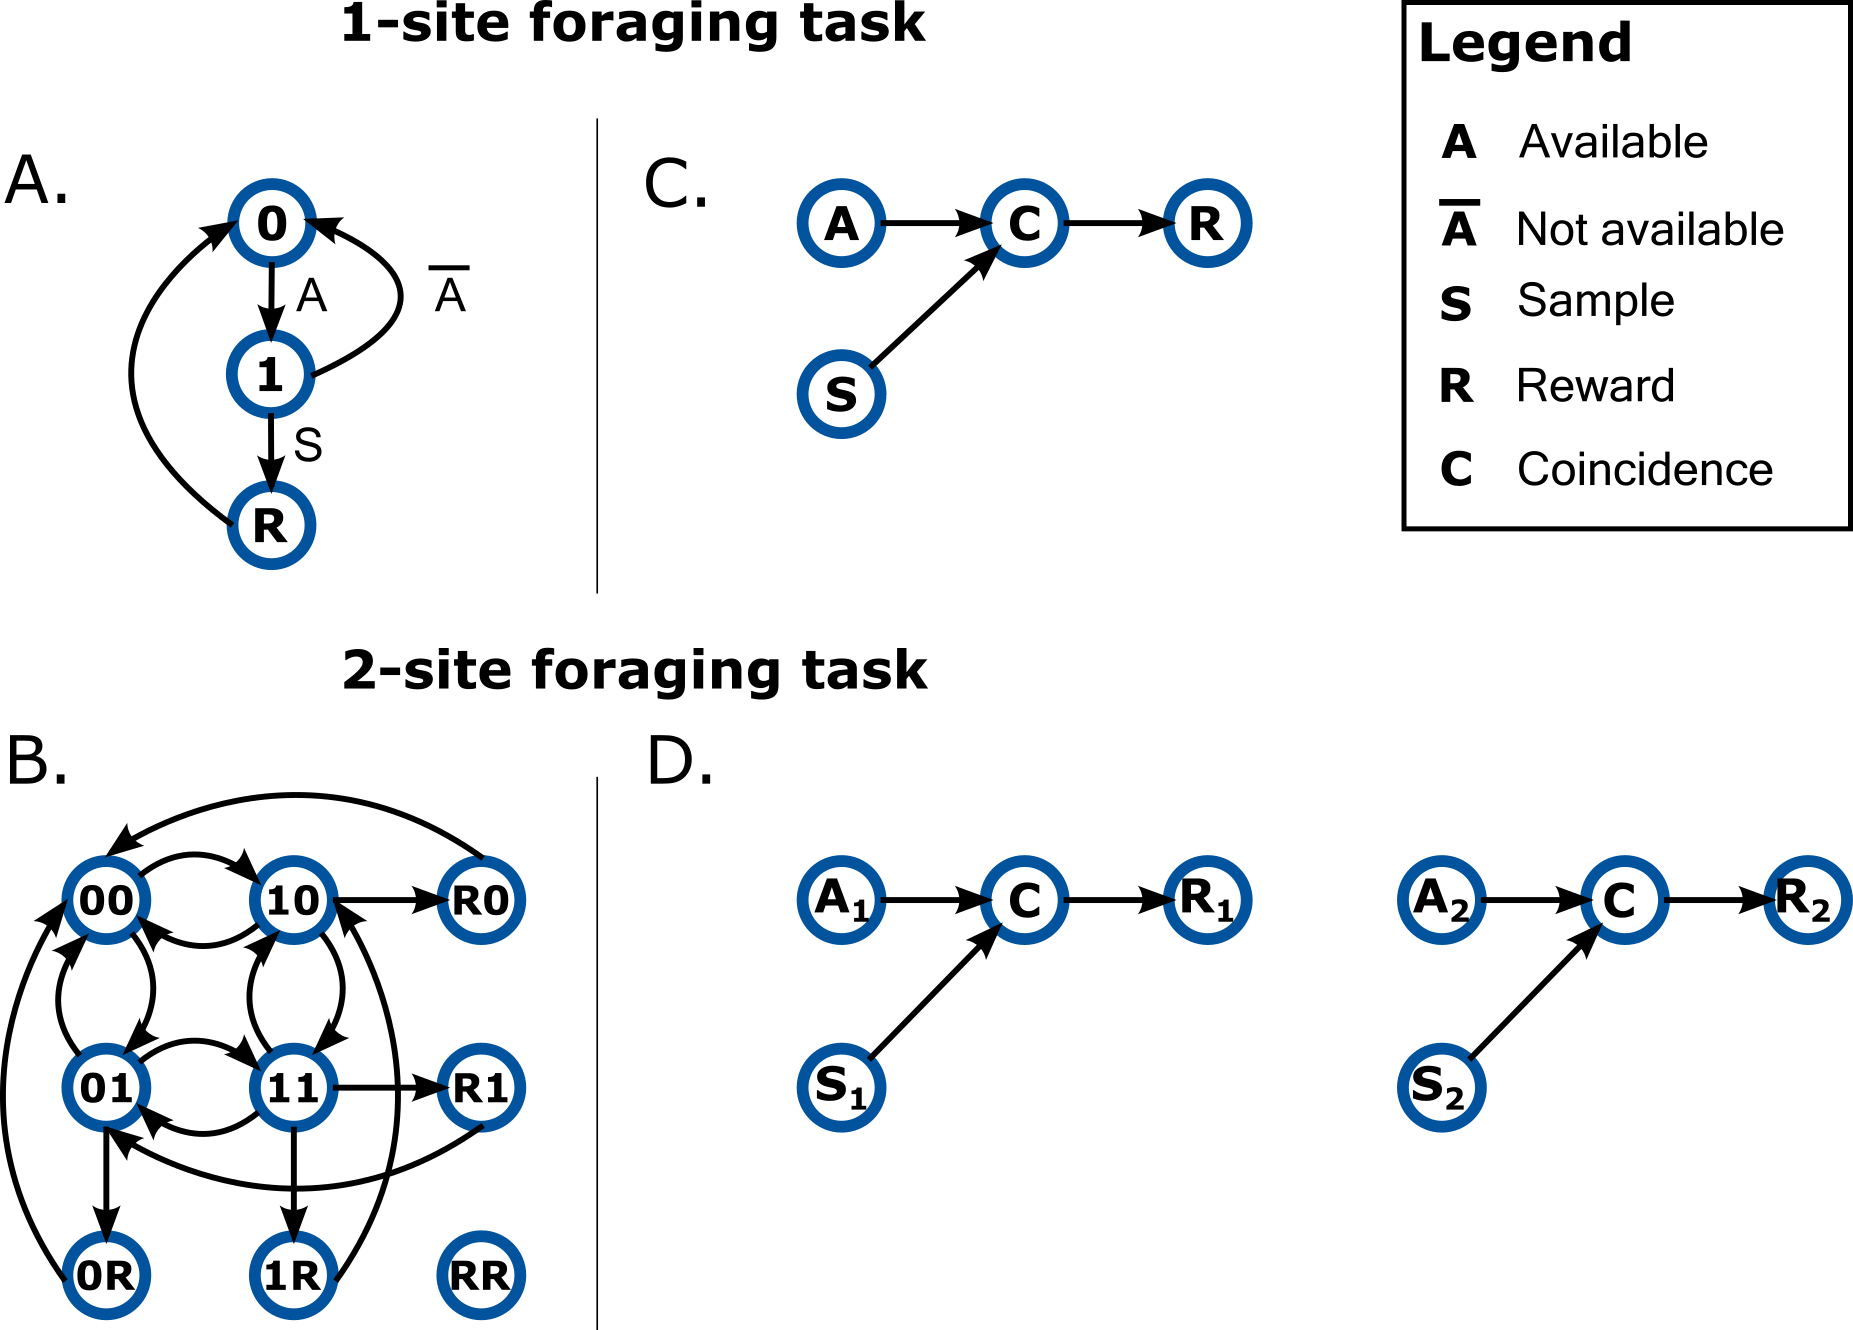
\includegraphics[width=\linewidth]{chapters/figuresChTools/bonsaiStateMachine}}
\end{center}
\vspace{-5mm}
\caption{Describing the behaviour of dynamic environments using either state-machines or dataflows.}
\label{fig:bonsaiStateMachine}
\end{figure}

How would designing such a scenario feel like in a reactive programming language? Figure \ref{fig:bonsaiStateMachine}C shows a possible specification of the 1-site foraging task in reactive terms. In this case, we have two sources of events from the environment: one timer signaling the availability of reward (A); and a sampling event (S) which is triggered every time the animal checks the location for food. Both of these events can occur independently of each other, but when a sampling event coincides with reward availability (C), then reward (R) is delivered. Because this description is intrinsically asynchronous and parallel, it makes it extremely easy to scale the task to a larger set of locations: just replicate the dataflow for each of the other locations (Figure \ref{fig:bonsaiStateMachine}D). In this example, the design space was made more intuitive by introducing the parallel and asynchronous nature of a real-world situation into our modeling formalism.

Another difficulty of the classical state machine formalism is dealing with continuous variables. The natural environment provides constant real-time feedback that tightly correlates with the actions of an animal. Reproducing such closed-loop interaction and manipulating its dynamics is a necessary tool for fully investigating brain function. Such models are virtually impossible to represent in a machine of finite states, given the potential infinitude of feedback responses. However, the dataflow formalism of asynchronous event sources can easily accommodate such models. In fact, this is their natural battleground; nodes represent reactive operators that promptly respond to input values broadcasted by event sources. These models of asynchronous computation are thus ideal for recreating the complex discrete and continuous aspects of natural environments that brains evolved to master. We thus propose Bonsai as a new tool for neuroscientists trying to understand how the brain deals with real world complexity.
